\documentclass[12pt]{article}
\usepackage{geometry}
\usepackage{amsmath,amssymb}
\usepackage{graphicx}
\usepackage{csquotes}
\usepackage{physics}
\usepackage{natbib}
\usepackage{enumitem}
\usepackage{subcaption}

\geometry{left=2cm, right=2cm}

\DeclareMathOperator{\E}{\mathbb{E}}
\newcommand{\refeq}[1]{Eq.~(\ref{#1})}
\usepackage{listings}
\usepackage{xcolor}

\definecolor{codegreen}{rgb}{0,0.6,0}
\definecolor{codegray}{rgb}{0.5,0.5,0.5}
\definecolor{codepurple}{rgb}{0.58,0,0.82}
\definecolor{backcolour}{rgb}{0.95,0.95,0.92}

\lstdefinestyle{mystyle}{
    backgroundcolor=\color{backcolour},   
    commentstyle=\color{codegreen},
    keywordstyle=\color{magenta},
    numberstyle=\tiny\color{codegray},
    stringstyle=\color{codepurple},
    basicstyle=\ttfamily\footnotesize,
    breakatwhitespace=false,         
    breaklines=true,                 
    captionpos=b,                    
    keepspaces=true,                 
    numbers=left,                    
    numbersep=5pt,                  
    showspaces=false,                
    showstringspaces=false,
    showtabs=false,                  
    tabsize=2
}

\lstset{style=mystyle}

\author{Chia-wei, Chen\thanks{R10323045}}
\title{HW1 \\ Labor Economics}


\begin{document}

\begin{titlepage}
    \maketitle
\end{titlepage}

\section{Setups}

 
\subsection{Data Camp}

I completed the course by taking the quiz. 
\begin{figure}[h]
  \centering
  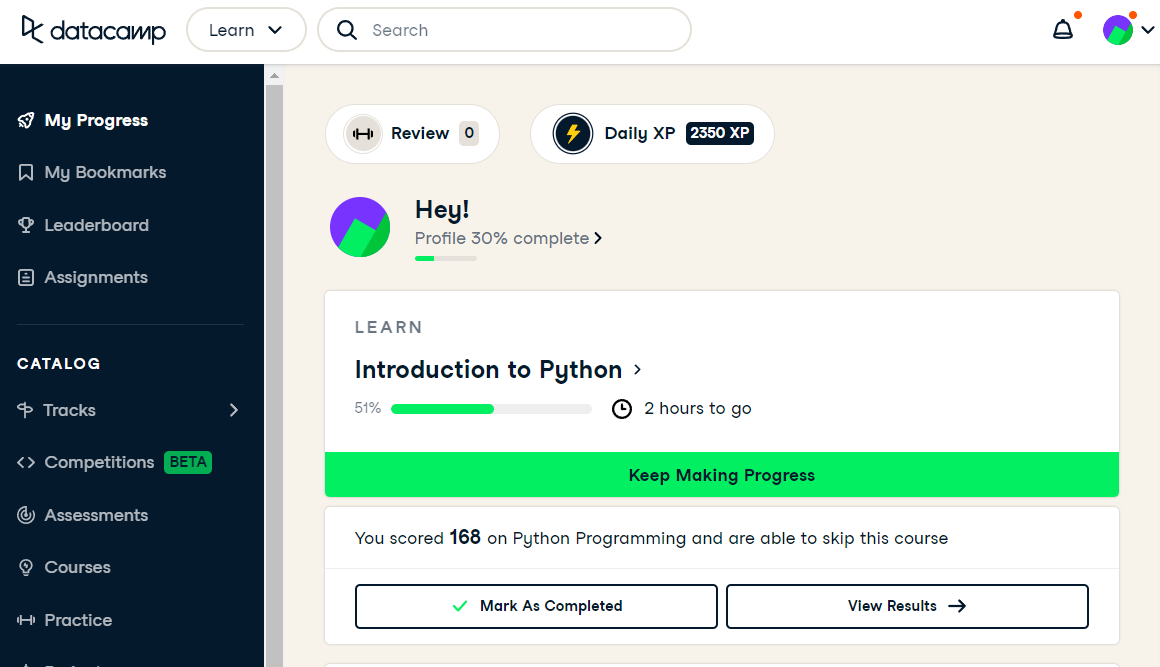
\includegraphics[width=0.5\textwidth]{image/Datacamp.png}
  \caption{Quiz in datacamp}
  \label{fig:data_camp}
\end{figure}
\subsection{R}

As shown in Figure~\ref{fig:R_setting}

\begin{figure}[h]
    \centering
    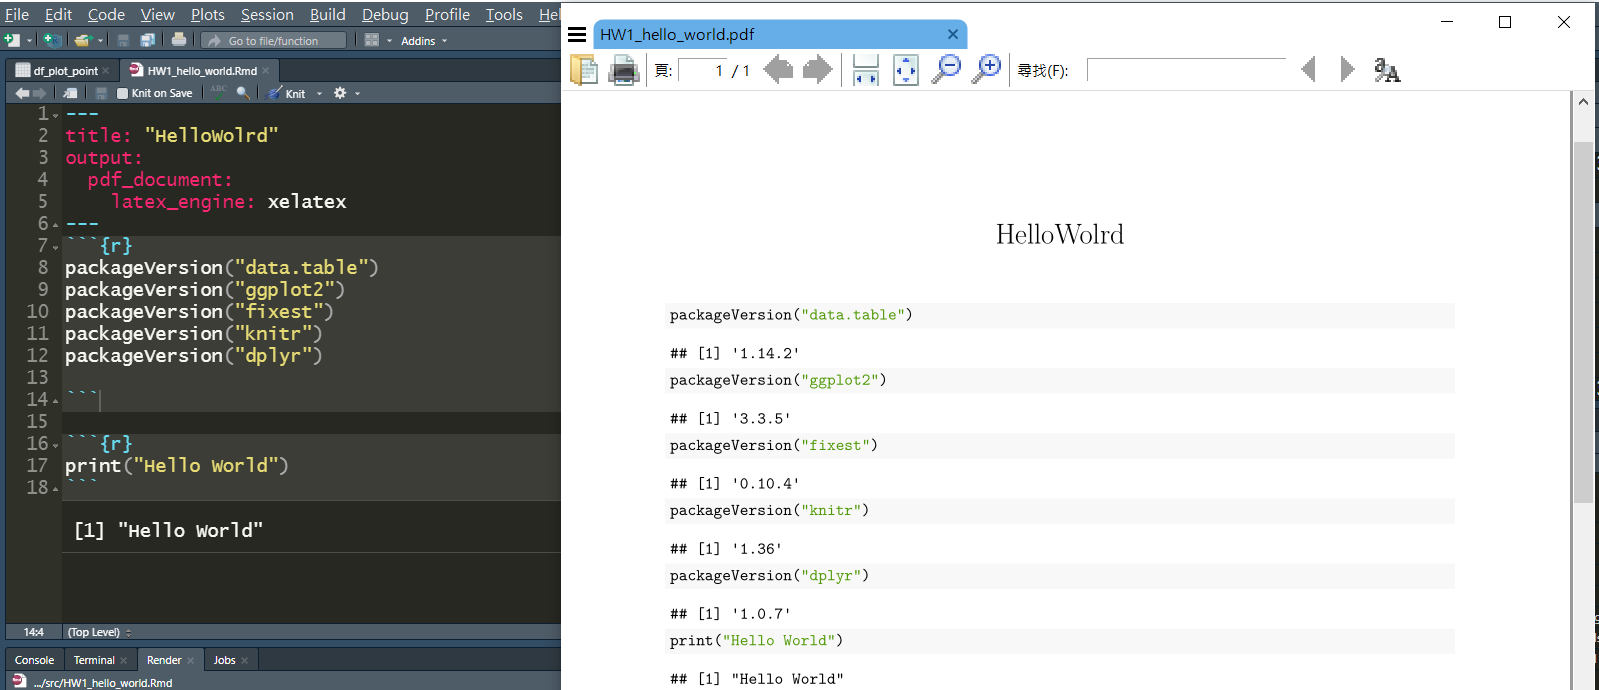
\includegraphics[width=0.9 \textwidth]{image/R.png}
    \caption{Settings and the libraries}
    \label{fig:R_setting}
\end{figure}
\subsection{Debugger}

\begin{figure}[h]
    \centering
    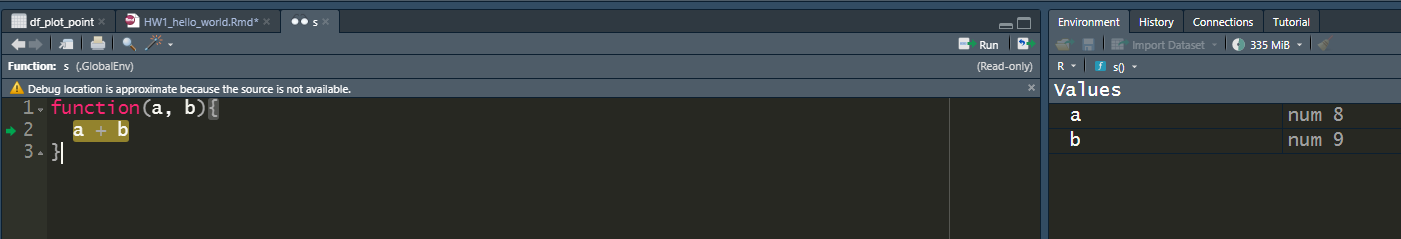
\includegraphics[width=0.9\textwidth]{image/debugger.png}
\end{figure}
\subsection{GitHub Setting}

I created a repository for the whole lecture instead. 
See figure~\ref{fig:github}

\begin{figure}[h]
    \centering
    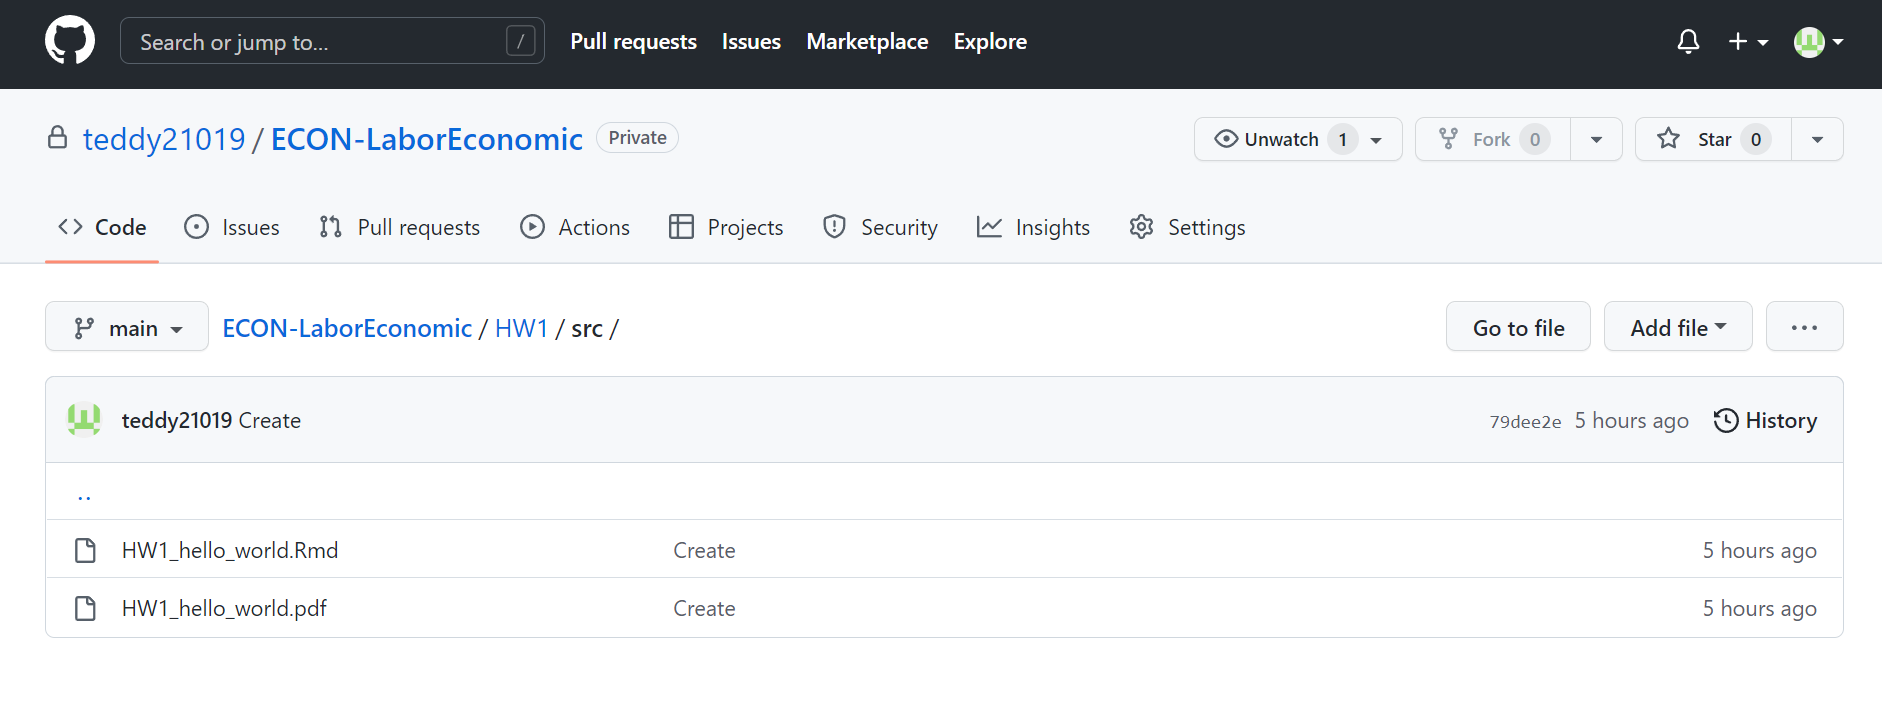
\includegraphics[width = 0.9\textwidth]{image/github.png}
    \caption{Github page, with the hello world files pushed on it}
    \label{fig:github}
\end{figure}

\section{NBER Working Paper}
\subsection{List paper on NBER}

The second paper on the list is 

\begin{displayquote}
    KFstar and Portfolio Inflows: A Focus on Latin America 

    by Burger, John D and Warnock, Francis E and Warnock, Veronica Cacdac
\end{displayquote}

\subsection{Download a Paper}
As in figure~\ref{fig:download_nber}, I downloaded the paper.

\begin{figure}[h]
    \centering
    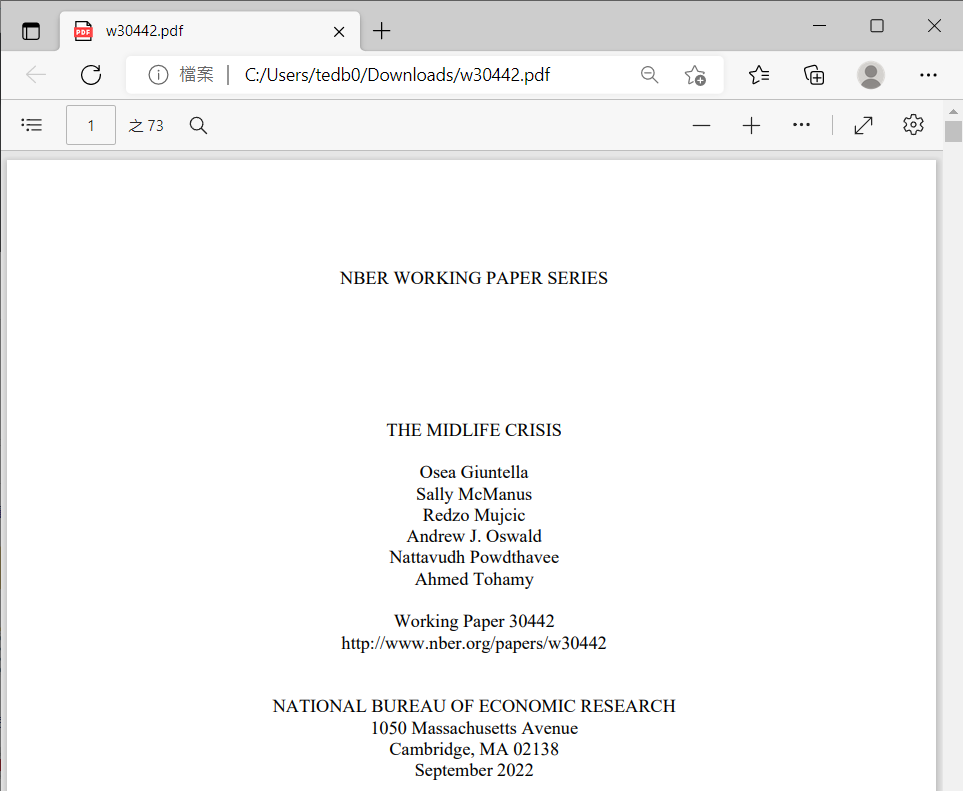
\includegraphics[width = 0.8\textwidth]{image/NBER_2.png}
    \caption{Screenshoe - paper downloaded}
    \label{fig:download_nber}
\end{figure}



\section{SRDA}
\subsection{SRDA Account}

The account info is shown in figure~\ref{fig:SRDA_acc}


\subsection{Plotting Rate of Working - Age from PSFD Data}

Plot as well as the year is shown in figure~\ref{fig:PSFD}



\begin{figure}
    \centering
    \begin{minipage}[t]{.5\textwidth}
        \centering
        
\includegraphics[width = \linewidth]{image/SRDA.png}
        \caption{Account info of SRDA}
        \label{fig:SRDA_acc}
    \end{minipage}%
    \begin{minipage}[t]{.5\textwidth}
        \centering
        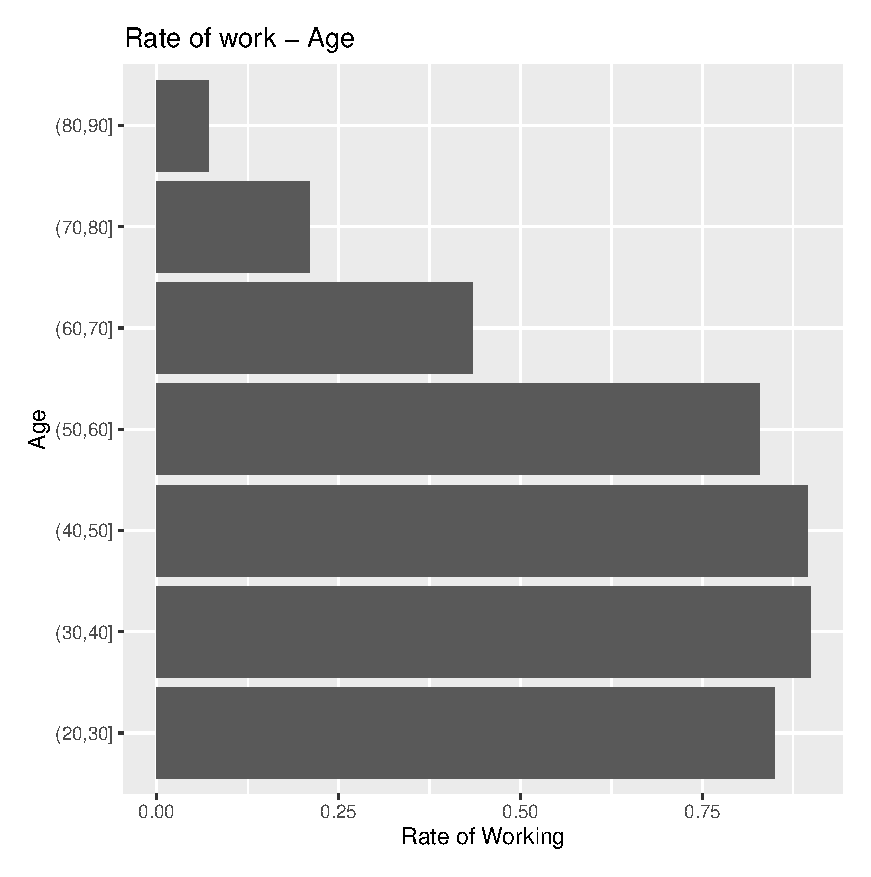
\includegraphics[width = 0.8\linewidth]{src/SRDA/Result/Work_age.eps}
        \caption{Rate of Working Versus the Age. Data source: PSFD 2000}
        \label{fig:PSFD}
    \end{minipage}
\end{figure}

\section{Roy Model}
\subsection{Theoretical Results}

\subsubsection{Derivation}

We first start from considering the probability of migration. 
One migrates under the condition

\begin{equation}
    w_{1i} > w_{0i} + C
\end{equation}

Where $w_{0i} = \mu_{0i} + \epsilon_0$ and $w_{1i} = \mu_{1i} + \epsilon_1$, 
and the error terms together follow a joint-normal distribution

\begin{equation}
    \label{eq:def_w}
    \mqty(\epsilon_0 \\ \epsilon_1) 
    \sim
    \mathcal{N} \qty(
        \mqty(0 \\ 0),
        \mqty(\sigma_0^2, \sigma_{01} \\
              \sigma_{01}, \sigma_1^2)
    )
\end{equation}

The probability of migration is then, according to \refeq{eq:def_w}

\begin{align}
    P(w_{1i} > w_{0i} + C) &= P(v_i > \mu_0 - \mu_1 + C) \nonumber \\
    &=1 - \Phi(\frac{\mu_0 - \mu_1 + C}{\sigma_\nu}) \nonumber \\
    &=1 - \Phi(z) \nonumber
\end{align}

The expected wage of an immigrant is then

\newcommand{\given}{\mid}

\emph{Note: Subscripts i are neglected for simplicity}
\begin{align*}
    \E(w_{0} \given I) =& \E(w_{0} \given v > \mu_0 - \mu_1 + C)  \\
    =& \mu_0 + \E(\epsilon_0 \given  v > \mu_0 - \mu_1 + C )  \\
    =& \mu_0 + \E \left(
            \epsilon_0 \given \frac{\nu}{\sigma_\nu} > \frac{\mu_0 - \mu_1 + C}{\sigma_\nu}
            \right)
\end{align*}

A linear combination of random variables following normal distribution
also follows a normal distribution. Therefore $\E\left(\epsilon_0 \given \frac{\nu}{\sigma_\nu}\right)$
is just a conditional expectation of a bivariate normal distribution
consisting $\epsilon$ and $\nu/\sigma_\nu$.

Since for a bivariate normal distribution, we have 
\begin{equation}
    \label{eq:biv-exp}
    \E[X \given Y=y] = \mu_x + \rho_{xy}\frac{\sigma_x}{\sigma_y}(y - \mu_y) 
\end{equation}

Substituting $X=\epsilon_0$ and $Y=\nu$ into \refeq{eq:biv-exp}, we get

\begin{equation}
    \label{eq:biv_normal_exp_0}
    \E(\epsilon_0 \given \nu)=\rho_{0\nu}\frac{\sigma_0}{\sigma_\nu}\nu
\end{equation}

and hence

\begin{equation*}
    \E(\epsilon_0 \given \frac{\nu}{\sigma_\nu})=
    \left(\rho_{0\nu} \frac{1}{\sigma_\nu}\right)
    \frac{\sigma_0}{\sigma_\nu \frac{1}{\sigma_\nu^2}}
    \frac{\nu}{\sigma_\nu}=\frac{\rho_{0\nu}\sigma_0 }{\sigma_\nu}\nu
\end{equation*}

Therefore
\begin{align}
    \E(w_{0} \given I) =& 
     \mu_0 + \E \left(
            \epsilon_0 \given \frac{\nu}{\sigma_\nu} > \frac{\mu_0 - \mu_1 + C}{\sigma_\nu}
            \right) \nonumber \\
    &= \mu_0 + \rho_{0\nu}\sigma_0 \E \left(
        \frac{\nu}{\sigma_\nu} 
        \given
        \frac{\nu}{\sigma_\nu} > \frac{\mu_0 - \mu_1 + C}{\sigma_\nu}
    \right) \label{eq:before_trunc}
\end{align}

Observe that the last expectation \refeq{eq:before_trunc}
is the expected value of a truncated normal distribution, 
which can be rewritten as 

\begin{equation}
    \label{eq:exp_wo_1}
    \E(w_{0} \given I) = 
    \mu_0 + \rho_{0\nu}\sigma_0 \frac{\phi(z)}{1-\Phi(z)}
\end{equation}

Since the correlation coefficient can be negative,
we know nothing about this result. 
Let us precede and solve for $\rho_{0\nu}$ 
further for better insight. 


\begin{equation*}
    \rho_{0v} = \frac{\sigma_{0\nu}}{\sigma_0\sigma_\nu}
\end{equation*}
\begin{equation}
    \label{eq:cov_0_nu}
    \sigma_{0\nu}=cov(\epsilon_0, \nu)=\E(\epsilon_0 (\epsilon_1 - \epsilon_0)) = \sigma_{01}-\sigma_0^2
\end{equation}

Substitute the result from \refeq{eq:cov_0_nu} and $\rho_{01}=\sigma_{01}/\sigma_0\sigma_1$, 
\refeq{eq:exp_wo_1} now becomes
\begin{equation}
    \label{eq:E_0_I}
    \E(w_{0} \given I) = 
    \mu_0 + \frac{\sigma_{01}-\sigma_0^2}{\sigma_\nu} \frac{\phi(z)}{1-\Phi(z)}
    =\mu_0 + \frac{\sigma_0 \sigma_1}{\sigma_\nu}\left(
        \rho - \frac{\sigma_0}{\sigma_1}
    \right)\frac{\phi(z)}{1-\Phi(z)}
\end{equation}

Similarly, for $\E(w_1 \given I)$, we have

\begin{align*}
    \E(w_{1} \given I) =& \E(w_{1} \given v > \mu_0 - \mu_1 + C)  \\
    =& \mu_1 + \E(\epsilon_1 \given  v > \mu_0 - \mu_1 + C )  \\
    =& \mu_1 + \E \left(
            \epsilon_1 \given \frac{\nu}{\sigma_\nu} > \frac{\mu_0 - \mu_1 + C}{\sigma_\nu}
            \right)
\end{align*}

Substituting 1 for 0 in \refeq{eq:biv_normal_exp_0}, we get
\begin{equation}
    \label{eq:biv_normal_exp_1}
    \E(\epsilon_1 \given \frac{\nu}{\sigma_\nu})
    =\frac{\rho_{1\nu}\sigma_1}{\sigma_\nu}\nu
\end{equation}

\refeq{eq:cov_0_nu} now becomes
\begin{equation}
    \label{eq:cov_1_nu}
    \sigma_{1\nu}=cov(\epsilon_, \nu)=
    \E(\epsilon_1 (\epsilon_1 - \epsilon_0)) = \sigma_{1}^2-\sigma_{01}
\end{equation}

Hence together we get
\begin{equation}
    \label{eq:E_1_I}
    \E(w_{1} \given I) = 
    \mu_1 + \rho_{1\nu}\sigma_1 \frac{\phi(z)}{1-\Phi(z)}
    =\mu_1 + \frac{\sigma_0 \sigma_1}{\sigma_\nu}\left(
        \frac{\sigma_1}{\sigma_0} - \rho
    \right)\frac{\phi(z)}{1-\Phi(z)}
\end{equation}



\subsubsection{$Q_0>0$ and $Q_1<0$ ?}\label{sec:imposible_case}

According to \refeq{eq:E_0_I} and \refeq{eq:E_1_I}, this would imply that
$$
\begin{cases}
    \rho>\frac{\sigma_0}{\sigma_1}\\
    \rho>\frac{\sigma_1}{\sigma_0}
\end{cases}
$$
But one will exceed 1, making it mathematically impossible to happen since correlation coefficient must be bounded under 1.
\begin{equation*}
    \rho > \max{\frac{\sigma_0}{\sigma_1},\frac{\sigma_1}{\sigma_0}} \ge 1
\end{equation*}
Intuitively, it means that people migrate to a place where expectation wage is lower than that in local.
which is weird and irrational.

\section{Simulation}
\subsection{Simulation}
\subsubsection{The code}
\lstinputlisting[language=R]{src/row_model_sim.R}


\subsubsection{Simulation Result}
% latex table generated in R 4.1.1 by xtable 1.8-4 package
% Mon Sep 19 12:52:20 2022
\begin{table}[ht]
\centering
\begin{tabular}{rrr}
  \hline
 & Wage.in.source & Wage.in.host \\ 
  \hline
1 & 9.22 & 17.05 \\ 
  2 & 9.22 & 17.04 \\ 
   \hline
\end{tabular}
\caption{Simulation result versus the theoretical result} 
\label{tab:sim_res}
\end{table}


\section{Roy Model is Everywhere}
\subsection{Example in Applied Economics}

A phenomenal example is that published by~\cite{Heckman76}. 
He estimates the labor supply and wage for females. 
Not only does the model handles the self-selection problem, it also provides 
a faster method for estimation, compared to his similar work in 
\citep[see][]{Heckman74}  



\subsection{Write Down a Research Question}

I found the concept of self selection extremely useful in explaining 
"Who take courses that are not in its own department?"

Similar to immigrants and wages, I found an analogy between students and grades.
Back when I was in the department of physics, some classmates tend to take
calculus and linear algebra in the department of mathematics, instead of the
equivalent required course in the department of physics. Those courses are typically
hard and has a relatively higher proportion of people failing. 

Meanwhile, people like me tend to take the so called "sweet courses", which 
guarantees a good grade, with little need for effort.

Assume that in average, taking courses in one's own department (Denoted $0$) will get a grade $\mu_0$
, while taking courses in other department (Denoted $1$) will get a grade $\mu_1$.
Also assume for now that the personalities of teachers are irrelevant, as well as the interest of individual student; 
that is, they only seek for a better score.


\subsection{Explanation}
Taking a direct analogy from the immigrants' problem, we know that 
\begin{enumerate}[label = Case \arabic{enumi}.]
    \item Students that take other courses are both getting better score than average.
    This refers to $Q_0>0$ and $Q_1>0$.
    This happens when $\sigma_1 > \sigma_0$ and $\rho>\frac{\sigma_0}{\sigma_1}$

    If the courses are relevant, for example, \emph{Advanced Linear Algebra} and \emph{Applied Mathematics(I)}
    \footnote{Mainly covering linear algebra as well}, and the distribution of grades in \emph{Advance Linear Algebra} is more 
    diverse, then students that are smarter take the other course, mainly because in a course that everyone takes A+(The easier \emph{Applied Mathematics}), 
    a small mistake might cause the grade to drop, while in the harder \emph{Advanced Linear Algebra}, almost all the 
    other classmates are noobs, and hence even a relatively big mistake in the exam doesn't change ones' good result much.

    \item Students that take other courses suck at both courses.
    This refers to $Q_0<0$ and $Q_1<0$.
    This happens when $\sigma_1 < \sigma_0$ and $\rho>\frac{\sigma_1}{\sigma_0}$

    In contrast to case 1, if taking course in the other department which is relevant has a more steady grade 
    (obviously not F), then students not performing well in either class will take the one in which the grade don't 
    fluctuate too much, preventing an unexpected failure that unfortunately might postpone its graduation year.

    \item Students that take other courses that they are good at.
    This refers to $Q_0<0$ and $Q_1>0$.
    This happens when $\rho<\min{\frac{\sigma_1}{\sigma_0},\frac{\sigma_0}{\sigma_1} }$

    If the two courses are less irrelevant, like \emph{Classical Electrodynamic Theory} and 
    \emph{Macroeconomics Theory}, then the students that take the course in the department of economics
    are the students that perform better in the other field of knowledge. 

    That's how I ended up here.

    \item Students that take other courses that they are not good at.
    This refers to $Q_0>0$ and $Q_1<0$. 
    This is mathematically impossible. Refer to section \ref{sec:imposible_case}.

    These are the irrational students, trying to challenge their limits and not thinking thoroughly.


\end{enumerate}


\pagebreak
\bibliographystyle{apa}
\bibliography{ref}

\end{document}